\documentclass[10pt,mathserif]{beamer}
\usepackage[T5]{fontenc}
\usepackage{fontspec}
\setsansfont{Segoe UI}
%\setmainfont{Segoe UI}
\usepackage[utf8]{inputenc}
% Style
\usepackage{graphicx,amsmath,amssymb,tikz,psfrag,amsthm,enumerate}
\usepackage[backend=biber,style=numeric,citestyle=ieee]{biblatex}

% ~~~~~~~~~~~~ Custom ~~~~~~~~~~~~
\usepackage{array}
\usepackage[parfill]{parskip}
%\usepackage{caption}
%\captionsetup[figure]{labelformat=empty}
%\usepackage{subcaption}
\usepackage{bm}
 \usepackage{amsfonts,amscd}
\usepackage{gensymb}
\usepackage[]{units}
\usepackage{listings}
\usepackage{multicol}
\usepackage{tcolorbox}
% -- \usepackage{physics}
\usepackage{ulem}
% ~~~~~~~~~~~~ Custom ~~~~~~~~~~~~
\graphicspath{{images/}}
\usepackage{hyperref}

% ~~~~~~~~~~~
%new commands
\newcommand{\der}[2]{\frac{d#1}{d#2}}
\newcommand{\nder}[3]{\frac{d^#1 #2}{d #3 ^ #1}}
\newcommand{\pder}[2]{\frac{\partial #1}{\partial #2}}
\newcommand{\npder}[3]{\frac{\partial ^#1 #2}{\partial #3^#1}}
\newcommand{\sentencelist}{def}
\newcommand{\overbar}[1]{\mkern 1.5mu\overline{\mkern-1.5mu#1\mkern-1.5mu}\mkern 1.5mu}
\newcommand{\lined}{\overbar}
\newcommand{\perm}[2]{{}^{#1}\!P_{#2}}
\newcommand{\comb}[2]{{}^{#1}C_{#2}}
\newcommand{\intall}{\int_{-\infty}^{\infty}}
\newcommand{\Var}[1]{\text{Var}\left(#1\right)}
\newcommand{\E}[1]{\text{E}\left(#1\right)}
\newcommand{\define}{\equiv}
\newcommand{\diff}[1]{\mathrm{d}#1}
\newcommand{\empy}[1]{{\color{darkorange}\emph{#1}}}
\newcommand{\empr}[1]{{\color{cardinalred}\emph{#1}}}

%\logo{\includegraphics[height=0.6cm]{hcmus}}

% ~~~~~~~~~~~~ Custom ~~~~~~~~~~~~

\input defs.tex

%% formatting
\mode<presentation>
{
\usetheme{default}
%\usetheme{Berlin}
\useinnertheme{circles}
}
\setbeamertemplate{navigation symbols}{}
\usecolortheme[rgb={0.13,0.28,0.59}]{structure}
%\setbeamertemplate{itemize subitem}{--}
\setbeamertemplate{frametitle} {
	\begin{center}
	  {\large\bf \insertframetitle}
	\end{center}
}

\newcommand\footlineon{
  \setbeamertemplate{footline} {
    \begin{beamercolorbox}[ht=2.5ex,dp=1.125ex,leftskip=.8cm,rightskip=.6cm]{structure}
      \footnotesize \insertsection
      \hfill
      {\insertframenumber}
    \end{beamercolorbox}
    \vskip 0.45cm
  }
}
\footlineon

\AtBeginSection[] 
{ 
	\begin{frame}<beamer> 
		\frametitle{Outline} 
		\tableofcontents[currentsection,currentsubsection] 
	\end{frame} 
} 

%% begin presentation

\title{\large \bfseries OpenHuman: The synthesis system for conversational gestures based on emotion and semantics}

\author{Thanh Hoang-Minh\\[2ex]
Giảng viên hướng dẫn: \\ TS. Lý Quốc Ngọc}
%University of Science

%\author{Your Name \\ Advisor: Professor Name}

\institute{
	\includegraphics[height=2cm]{hcmus.png}\\
	Faculty of Information Technology\\
	VNUHCM-University of Science}
\date{\today}

\begin{document}

%\begin{frame}[plain]
%	\titlepage
%\end{frame}

\frame{
\thispagestyle{empty}
\titlepage
}

% ~~~~~~~~~~~~~~~~~~~~~~~~~~~~~~~~~~~~~~~~
\section{Minh hoạ}

%\begin{frame}
%	
%\end{frame}

\begin{frame}{Minh hoạ quá trình sinh cử chỉ}
	\vspace{10pt}
	\begin{columns}
		\begin{column}{0.7\textwidth}
			\begin{itemize}
				\item Sinh cử chỉ (Gesture Generation) là gì?
				
				\begin{figure}[h]
					\centering
					\includegraphics[width=\textwidth]{GestureGenerationExplain}
				\end{figure}
			
%				\item Mục tiêu của việc sinh cử chỉ?
%					\begin{quote}
%					"The goal of Gesture Generation is to generate gestures that are natural, realistic, and appropriate for the given context."
%				\end{quote}
			\end{itemize}
			ACM CCS: • Human-centered computing → Human computer interaction (HCI).
			
		\end{column}
		\begin{column}{0.3\textwidth} % Right column for image
			\begin{figure}[h]
			\centering
			\includegraphics[height={6cm}]{SampleAnimation}
			
%				\begin{quote}
%					{\tiny
%					"Your work is gonna fill a large part of your life . And the only way to be truly satisfied is to do what you believe is great work and the only way to do great work is to love what you do."}
%				\end{quote}
				
			{
			\small Demo Gesture Generation: \href{https://www.youtube.com/watch?v=B6nv1kQmi-Q}{\textcolor{blue}{\uline{Youtube}}}
			}
			\end{figure}
		\end{column}
	\end{columns}
\end{frame}

%\begin{frame}
%\frametitle{Bulleted list}
%\begin{itemize}\itemsep=12pt
%\item XXX
%\vspace*{0.5em}
%\begin{itemize}
%\item XXX
%\item XXX
%\item XXX
%\end{itemize}
%\item XXX
%\vspace*{0.5em}
%\begin{itemize}
%\item XXX
%\item XXX
%\item XXX
%\end{itemize}
%\item XXX
%\end{itemize}
%\end{frame}

%\begin{frame}
%\frametitle{Pictures with tikz}
%\begin{center}
%\begin{tikzpicture}
%	[scale=1.5,dot/.style={circle,draw=black!100,fill=black!100,thick,inner sep=0pt,minimum size=2pt}]
%    \node[dot] at (-1,0) (n1) {};
%    \node[dot] at (0,1)  (n2) {};
%    \node[dot] at (1,0)  (n3) {};
%    \node[dot] at (0,-1) (n4) {};
%    \draw[gray] (-1.5,0) -- (1.5,0);
%    \draw[gray] (0,-1.5) -- (0,1.5);
%    \draw[black,thick] (n1) -- (n2) -- (n3) -- (n4) -- (n1) -- cycle;
%    \draw[orange,thick] (-1,0.5) -- (0,1) -- (1,1.5);
%\end{tikzpicture}
%\qquad
%\begin{tikzpicture}
%	[scale=1.5,dot/.style={circle,draw=black!100,fill=black!100,thick,inner sep=0pt,minimum size=2pt}]
%    \draw[gray] (-1.5,0) -- (1.5,0);
%    \draw[gray] (0,-1.5) -- (0,1.5);
%    \draw[black,thick] (-1,1) -- (0,0) -- (1,1);
%\end{tikzpicture}
%\end{center}
%\end{frame}


%\begin{frame}
%\frametitle{Pictures with tikz}
%\begin{itemize}\itemsep=12pt
%	\item convex envelope of (nonconvex) $f$ is the largest convex underestimator $g$
%    \item \ie, the best convex lower bound to a function
%        \vspace*{1em}
%\begin{center}
%\begin{tikzpicture}
%    \draw[gray] (-1.5,0) -- (1.5,0);
%    \draw[gray] (0,-0.5) -- (0,1.5);
%    \draw[black,thick] (-1,1) -- (0,0) -- (0.5,0.5) -- (1,-0.25) -- (2,1);
%    \draw[black,dashed] (0,0) -- (1,-0.25);
%\end{tikzpicture}
%\end{center}
%%    \item \textbf{example}: $\ell_1$ is the envelope of $\card$ (on unit $\ell_\infty$ ball)
%%    \item \textbf{example}: $\|\cdot\|_*$ is the envelope of $\rank$ (on unit spectral norm ball)
%%    \item various characterizations: \eg, $f^{**}$ or convex hull of epigraph
%\end{itemize}
%\end{frame}

% ~~~~~~~~~~~~~~~~~~~~~~~~~~~~~~~~~~~~~~~~
\section{Giới thiệu}

\begin{frame}{Động lực nghiên cứu}
	\vspace{5pt}
	
	\begin{columns}
	% Left column
	\begin{column}{0.7\textwidth}
		\textbf{Text-base Deep Learning}
		\begin{itemize}
			\item ChatGPT, Alexa, Character.AI,..
			\item Text to speech, text to text,..
		\end{itemize}
		
		\textbf{Text/audio to Realistic Digital Humam}
		
		\begin{itemize}
			\item Video-base (HeyGen, Midjourney,...)
			\item Rendering-base:
			\begin{itemize}
				\item Character model (Gaussian Splatting)
				\item Character animation: (3D keypoints)
			\end{itemize}
		\end{itemize}
		\vspace{5pt}
		\centering
		\includegraphics[width=0.8\textwidth]{FacialAsset.png}
	\end{column}
	
	% Right column
	\begin{column}{0.3\textwidth}
		\begin{figure}
				\includegraphics[width=\textwidth]{UniversalHuman.png}
%				\caption{\small Minh hoạ người kỹ thuật số siêu thật (realistic digital human)}
		\end{figure}
		
		\begin{figure}
			\includegraphics[width=\textwidth]{MetaHuman.jpg}
			\caption{\small Minh hoạ người kỹ thuật số siêu thật (realistic digital human)}
		\end{figure}
	
	\end{column}
	
	\end{columns}
\end{frame}



\begin{frame}{Dữ liệu bài toán}
	
	
	\begin{columns}
		
		\begin{column}{0.7\textwidth}
			
			\textbf{Kiến trúc khung xương}
			\begin{itemize}
				\item Chuỗi chuyển động khung xương
				\begin{itemize}
					\item Skeleton: 75 bones: $\mathbf{B} = \{ \mathbf{b}_i \}^{75} $ \\
					\small{(\texttt{Head}, \texttt{Spine}, \texttt{Hips}, \texttt{LeftArm},\texttt{RightArm}... )} \\
					Dữ liệu BVH: $\mathbf{b}_{i} = \{r_x, r_y, r_z\}$
				\end{itemize}
				\begin{figure}[h]
					\centering
					\includegraphics[width=0.9\textwidth]{BoneRotationSeries}
				\end{figure}
				
				\item Dữ liệu sau xử lý: $\mathbf{g} \in \mathbb{R}^{D}$, với $D=1141$ 
				$\mathbf{g} = \Big[ \mathbf{p},  \mathbf{r},
				\mathbf{ p }',  \mathbf{r}',
				\mathbf{p}_{\text{joins}},  \mathbf{r}_{\text{joins}},
				\mathbf{p}'_{\text{joins}},  \mathbf{r}'_{\text{joins}},
				\mathbf{d}_{\text{gaze}}
				\Big]$
			\end{itemize}
			\vspace{10pt}
			\textbf{Loại bài toán}: Hồi quy (regression)
			\begin{itemize}
				\item Cho trước $N$ khung hình (frame) cử chỉ, dự đoán $M$ khung hình tiếp theo tương ứng với âm thanh $\mathbf{a}$.
			\end{itemize}
		
		\end{column}
		
			\begin{column}{0.3\textwidth}
				\begin{figure}[h]
					\centering
					\includegraphics[width=\textwidth]{Skeleton}
				\end{figure}
		\end{column}
		
	\end{columns}
	
\end{frame}

\begin{frame}{Phát biểu bài toán}
%\frametitle{Group lasso \\[-0.3em] 
%{\footnotesize \textmd{(\eg, Yuan \& Lin; Meier, van de Geer, B\"uhlmann; Jacob, Obozinski, Vert)}}}


 \begin{figure}[h]
	\centering
	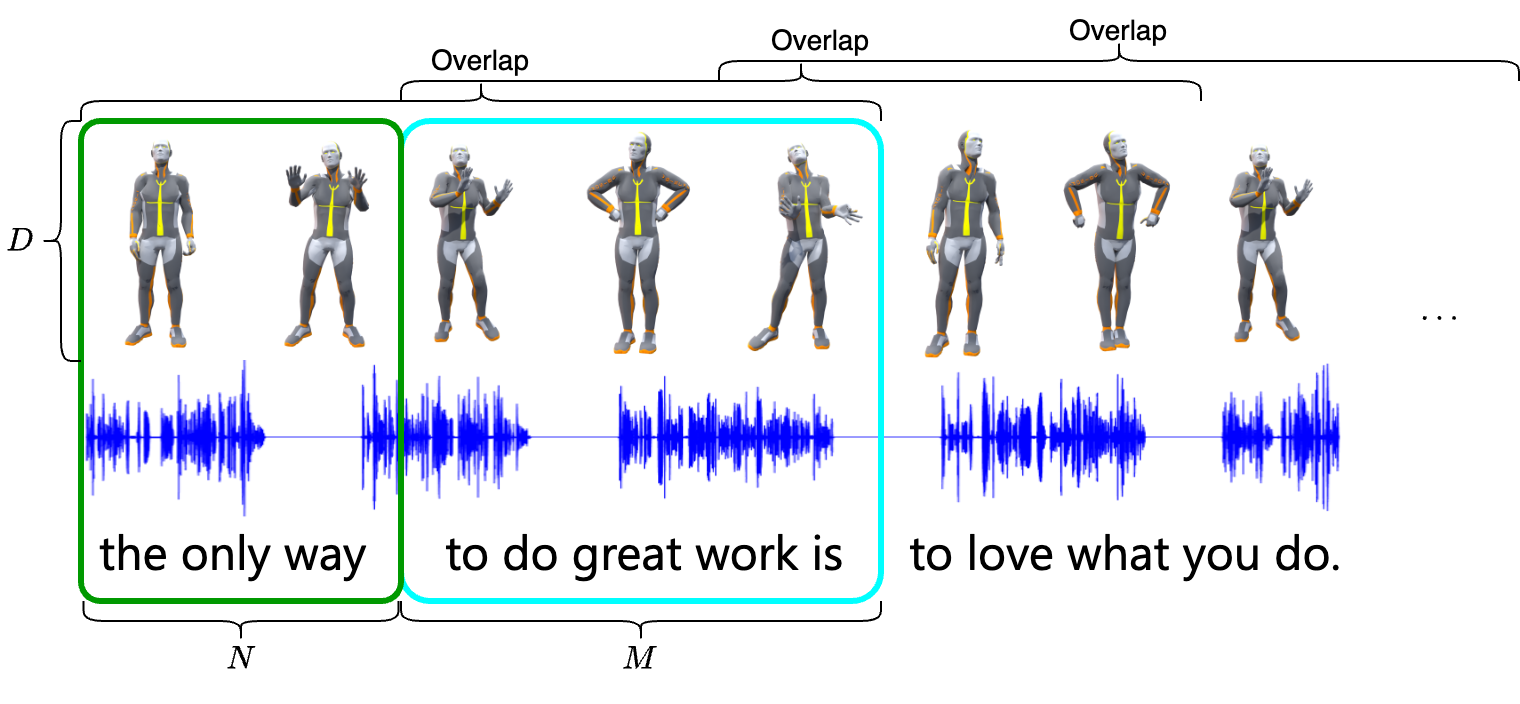
\includegraphics[height=4.5cm]{GestureSeries}
\end{figure}

\vspace{-10pt}

\begin{columns}
	
	\begin{column}{0.6\textwidth}
		
		\textbf{Input}
		\begin{itemize}
			\item Chuỗi cử chỉ khởi tạo: $\mathbf{g}_{0} \in \mathbb{R}^{N \times D}$
			\item Chuỗi âm thanh: $\mathbf{a}_{\text{raw}}$ sample rate 16000, trích xuất đặc trưng MFCC: $\mathbf{a} \in \mathbb{R}^{M \times 12}$
			\item Cảm xúc: $\mathbf{e} \in \mathbb{R}^6$ (\texttt{Happy},  \texttt{Sad}, \texttt{Angry},...)
		\end{itemize}
		
	\end{column}
	\begin{column}{0.4\textwidth}
		 \textbf{Output}
		 \begin{itemize}
		 	\item Chuỗi cử chỉ dự đoán: $\hat{\mathbf{x}} \in \mathbb{R}^{M \times D}$
		 \end{itemize}
		 
		 \textbf{Grouth Truth}
		 \begin{itemize}
		 	\item Chuỗi cử chỉ gốc: $ \mathbf{x}  \in \mathbb{R}^{M \times D}$
		 \end{itemize}
	\end{column}
\end{columns}

\end{frame}

\begin{frame}{Khung chương trình}
	
\textbf{Training}
	\begin{itemize}
		\item $f_{\theta}(\mathbf{g}_0, \mathbf{a}, \mathbf{e})$
	\end{itemize}

	
\textbf{Inference}

	\begin{itemize}
		\item $\mathbf{x}' = f_{\theta'}$
	\end{itemize}
\end{frame}

%\[
%\begin{array}{ll}
%\mbox{minimize} & f(x) + \lambda \sum_{i=1}^N \|x_i\|_2
%\end{array}
%\]


%\begin{frame}{Structured group lasso \\[-0.3em] 
%{\footnotesize \textmd{(Jacob, Obozinski, Vert; Bach et al.; Zhao, Rocha, Yu; \dots)}}}
%\begin{itemize}\itemsep=12pt
%\item problem:
%\[
%\begin{array}{ll}
%\mbox{minimize} & f(x) + \sum_{i=1}^N \lambda_i \|x_{g_i}\|_2
%\end{array}
%\]
%where $g_i \subseteq [n]$ and $\mathcal G = \{g_1, \dots, g_N\}$
%\item like group lasso, but the groups can overlap arbitrarily
%\item particular choices of groups can impose `structured' sparsity
%\item \eg, topic models, selecting interaction terms for (graphical) models,
%    tree structure of gene networks, fMRI data
%\item generalizes to the \textbf{composite absolute penalties family}:
%\[
%r(x) = \|(\|x_{g_1}\|_{p_1}, \dots, \|x_{g_N}\|_{p_N})\|_{p_0}
%\]
%\end{itemize}
%\end{frame}

%\begin{frame}{Structured group lasso \\[-0.3em] 
%{\footnotesize \textmd{(Jacob, Obozinski, Vert; Bach et al.; Zhao, Rocha, Yu; \dots)}}}
%\textbf{hierarchical selection}:
%\begin{center}
%\begin{tikzpicture}
%[dot/.style={rectangle,draw=black,fill=white,inner sep=5pt,minimum size=5pt}]
%\node[dot,draw=orange,thick] at (0,5) (n1) {1};
%\node[dot] at (-1,4) (n2) {2};
%\node[dot,draw=orange,thick] at (1,4) (n3) {3};
%\node[dot] at (-1,3) (n4) {4};
%\node[dot,draw=orange,thick] at (0.5,3) (n5) {5};
%\node[dot] at (1.5,3) (n6) {6};
%\draw[->] (n1) -- (n2);
%\draw[->] (n1) -- (n3);
%\draw[->] (n2) -- (n4);
%\draw[->] (n3) -- (n5);
%\draw[->] (n3) -- (n6);
%\end{tikzpicture}
%\end{center}
%\begin{itemize}\itemsep=8pt
%    \item $\mathcal G = \{ \{4\}, \textcolor{orange}{\{5\}}, \{6\}, \{2,4\}, 
%        \textcolor{orange}{\{3,5,6\}}, \textcolor{orange}{\{1,2,3,4,5,6\} \}}$
%\item nonzero variables form a rooted and connected subtree
%    \begin{itemize}
%        \item if node is selected, so are its ancestors
%        \item if node is not selected, neither are its descendants
%    \end{itemize}
%\end{itemize}
%\end{frame}

%\begin{frame}[fragile]{Sample ADMM implementation: lasso}
%\begin{verbatim}
%prox_f = @(v,rho) (rho/(1 + rho))*(v - b) + b;
%prox_g = @(v,rho) (max(0, v - 1/rho) - max(0, -v - 1/rho));
%
%AA = A*A';
%L  = chol(eye(m) + AA);
%
%for iter = 1:MAX_ITER
%    xx = prox_g(xz - xt, rho);
%    yx = prox_f(yz - yt, rho);
%
%    yz = L \ (L' \ (A*(xx + xt) + AA*(yx + yt)));
%    xz = xx + xt + A'*(yx + yt - yz);
%  
%    xt = xt + xx - xz;
%    yt = yt + yx - yz;
%end
%\end{verbatim}
%\end{frame}



%\begin{frame}{Algorithm}
%    if $L$ is not known (usually the case), can use the following line search:
%    \noindent\rule[-5pt]{\textwidth}{0.4pt}
%    {\footnotesize
%    \begin{tabbing}
%        {\bf Given} $x^k$, $\lambda^{k-1}$, and parameter $\beta \in (0,1)$. \\*[\smallskipamount]
%        Let $\lambda := \lambda^{k-1}$. \\*[\smallskipamount]
%        {\bf Repeat} \\
%        \qquad \= 1.\ Let $z := \prox_{\lambda g}(x^{k} - \lambda \nabla f(x^{k}))$. \\
%        \> 2.\ {\bf break if} $f(z) \leq \hat{f}_{\lambda}(z, x^{k})$. \\
%        \> 3.\ Update $\lambda := \beta \lambda$. \\*[\smallskipamount]
%        {\bf Return} $\lambda^{k} := \lambda$, $x^{k+1}:=z$.
%    \end{tabbing}}
%    \noindent\rule[10pt]{\textwidth}{0.4pt}
%
%    typical value of $\beta$ is $1/2$, and 
%    \[
%    \hat{f}_\lambda(x,y) = f(y) + \nabla f(y)^T (x - y) + 
%    (1/2\lambda)\|x - y\|_2^2
%    \]
%\end{frame}


\section{Công trình liên quan}

\begin{frame}{Các phương pháp}
	\textbf{Rule Base}
	\begin{itemize}
		\item BEAT
	\end{itemize}
	
	\textbf{Statistic}
	\begin{itemize}
		\item Gesture Controllers
	\end{itemize}
	
	\textbf{DeepLearning}
	\begin{itemize}
		\item Gesticulator (Multilayer perceptron), RNN(Speech2AffectiveGestures, HA2G, TransGesture, ..)
	\end{itemize}
	
\end{frame}

\section{Mô hình sinh cử chỉ}

\begin{frame}
	
	$x^{2} \in \mathbb{R}^{x \times y}$
\end{frame}

\section{Thực nghiệm}

\begin{frame}
	
	$x^{2} \in \mathbb{R}^{x \times y}$
\end{frame}

\section{Kết luận}

\begin{frame}
	
	$x^{2} \in \mathbb{R}^{x \times y}$
\end{frame}

\begin{frame}[label=frame]{Sample frame title}
	
	In this slide, some important text will be
	\alert{highlighted} because it's important.
	Please, don't abuse it.
	
	\begin{block}{Remark}
		Sample text
	\end{block}
	
	\begin{alertblock}{Important theorem}
		Sample text in red box
	\end{alertblock}
	
	\begin{examples}
		Sample text in green box. The title of the block is ``Examples".
	\end{examples}
	\hyperlink{appendix}{\beamerbutton{More on Appendix}}
\end{frame}


\end{document}
